\documentclass[11pt]{beamer}
\usetheme{Madrid}
\usefonttheme{serif}

\usepackage[utf8]{inputenc}       % Encoding
\usepackage[english]{babel}       % Language
\usepackage[T1]{fontenc}          % Font encoding

\usepackage{amsmath, amsfonts, amssymb} % Math packages
\usepackage{graphicx}
\usepackage{xcolor}
\usepackage{colortbl}
\usepackage{array}
\usepackage{subcaption}

\usepackage{tikz}
\usepackage{tikz-uml}
\usetikzlibrary{arrows.meta, positioning, calc}
\usepackage{blkarray}
\usepackage{pgfplots}
\pgfplotsset{compat=1.18}

% Code formatting
\usepackage{minted}
\usepackage{adjustbox}
\usepackage[ruled,vlined]{algorithm2e}
\SetKwProg{While}{while}{}{}
\SetKwProg{For}{for}{}{}
\SetKwProg{Function}{function}{}{}

% Custom math operators
\DeclareMathOperator{\sen}{sen}
\DeclareMathOperator{\tg}{tg}

% Numbered captions in figures/tables
\setbeamertemplate{caption}[numbered]

% Metadata
\author[Mathys Vinatier]{Mathys Vinatier}
\title{Optimized Kalman Filter}
\setbeamercovered{transparent}
\setbeamertemplate{navigation symbols}{}
\logo{\includegraphics[scale=.05]{../img/logoSNU.png}}
\institute[]{Seoul National University}
\date{\today}

% Bibliography
\usepackage{biblatex} 
\addbibresource{../references.bib}

%Glossary
\usepackage[acronym]{glossaries}
\makeglossaries
% glossary.tex (no preamble commands here)

\newacronym{PPO}{PPO}{Proximal Policy Optimizer}

\newacronym{ALS}{ALS}{Autocovariance Least-Squares}

\newacronym{FKF}{FKF}{Field Kalman Filter}

\newacronym{OKF}{OKF}{Optimized Kalman Filter}

\newacronym{NN}{NN}{Neural Network}

\newacronym{RNN}{RNN}{Recursive Neural Network}

\newacronym{LSTM}{LSTM}{Long Short-Term Memory}

\newacronym{MB}{MB}{Model Based}

\newacronym{KF}{KF}{Kalman Filter}

\newacronym{EKF}{EKF}{Extended Kalman Filter}

\newacronym{DD}{DD}{Data Driven}

\newacronym{KG}{KG}{Kalman Gain}

\newacronym{SS}{SS}{State Space}

\newacronym{MSE}{MSE}{Mean Square Error}

\newacronym{SPD}{SPD}{Symmetric Positive Definite}

\newacronym{WFA}{WFA}{Walk Forward Analysis}

\newacronym{TRPO}{TRPO}{Trust Region Policy Optimization}

\newacronym{LMA}{LMA}{Logarithmic Movement Average}

\newacronym{RL}{RL}{Reinforcement Learning}

\newacronym{MDP}{MDP}{Markov Decision Process}

\newacronym{API}{API}{Approximate Policy Iteration}

\newacronym{LR}{LR}{Logistic Regression}

\newglossaryentry{KalmanNet}{
    name={KalmanNet},
    description={Neural network-based model that integrates Kalman filtering techniques for improved state estimation in dynamic systems.}
}


\begin{document}
\begin{frame}
    \titlepage
\end{frame}
\begin{frame}{Epsilon-Greedy Policy}
\vfill
\begin{itemize}
    \item \textbf{Q-table:} Internally, Q-Learning uses a Q-table storing values for each state-action pair. Initially, all values are zero, and the table is updated iteratively during training.
\end{itemize}
\vfill
\[
    Q(s_t, a_t) \leftarrow Q(s_t, a_t) + \alpha \left[r_{t+1} + \gamma \max_{a} Q(s_{t+1}, a) - Q(s_t, a_t)\right]
\]
\vfill
\begin{center}
    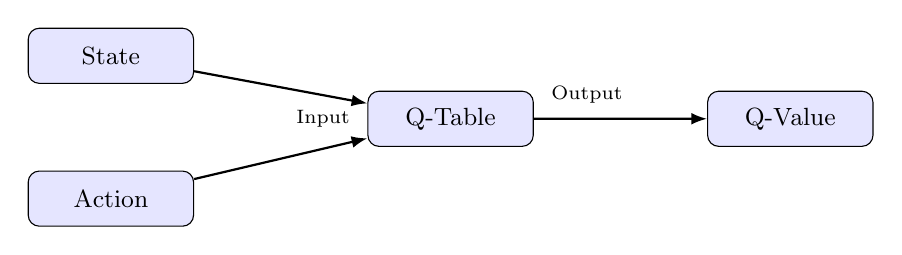
\begin{tikzpicture}[
        scale=0.7,
        node distance=1.1cm and 2.2cm,
        box/.style={draw, rounded corners, minimum width=2.1cm, minimum height=0.7cm, align=center, font=\small, fill=blue!10},
        arrow/.style={-{Latex[length=2mm]}, thick}
    ]
    % Nodes
    \node[box] (state) {State};
    \node[box, right=of state, yshift=-0.8cm] (qtable) {Q-Table};
    \node[box, below=of state] (action) {Action};
    \node[box, right=of qtable] (qvalue) {Q-Value};
    % Arrows
    \draw[arrow] (state) -- (qtable);
    \draw[arrow] (action) -- (qtable);
    \draw[arrow] (qtable) -- (qvalue);
    % Labels
    \node[left=1mm of qtable] {\scriptsize{Input}};
    \node[right=1mm of qtable, yshift=3mm] {\scriptsize{Output}};   
    \end{tikzpicture}
\end{center}

\vfill

\end{frame}

\begin{frame}{Epsilon-Greedy Policy}
    \vfill
    \begin{itemize}
        \item \textbf{Epsilon-Greedy Strategy :} To balance exploration and exploitation, actions are chosen using an epsilon-greedy policy
            \[
                \pi^*(s) = \arg\max_{a} Q^*(s, a)
            \]
    \end{itemize}
    \vfill
    \begin{center}
        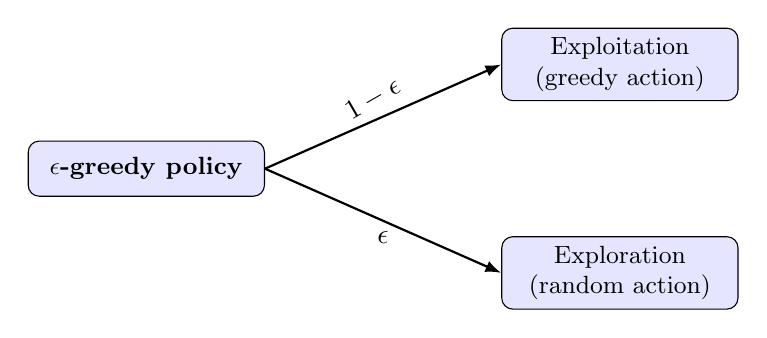
\begin{tikzpicture}[
        scale=0.5,
        node distance=0.5cm and 3cm,
        box/.style={draw, rounded corners, minimum width=3cm, minimum height=0.7cm, align=center, fill=blue!10, font=\small},
        arrow/.style={-{Latex[length=2mm]}, thick}
        ]
        % Nodes
        \node[box] (policy) {\textbf{$\epsilon$-greedy policy}};
        \node[box, above right=of policy] (exploit) {Exploitation\\(greedy action)};
        \node[box, below right=of policy] (explore) {Exploration\\(random action)};
        % Arrows
        \draw[arrow] (policy.east) -- node[above, pos=0.5, rotate=30] {$1-\epsilon$} (exploit.west);
        \draw[arrow] (policy.east) -- node[below, pos=0.5] {$\epsilon$} (explore.west);
        \end{tikzpicture}
    \end{center}
    \vfill
\end{frame}

\begin{frame}{Environement Implementation}
\begin{columns}[T]
    \begin{column}{0.48\textwidth}
        {\tiny
        \begin{tikzpicture}
        % TradingEnv class
        \umlclass[width=.95\linewidth, x=0, y=0]{TradingEnv}{
            - df : DataFrame \\
            - n\_steps : int \\
            - current\_step : int \\
            - initial\_balance : float \\
            - balance : float \\
            - position : int \\
            - last\_action : int \\
            - observation\_space : Box \\
            - action\_space : Discrete
        }{
            + \_\_init\_\_(df) \\
            + \_get\_obs() \\
            + sample\_valid\_action() \\
            + get\_valid\_actions() \\
            + step(action) \\
            + set\_data(df) \\
            + reset()
        }
        \end{tikzpicture}
        }
    \end{column}
    \begin{column}{0.52\textwidth}
        {\tiny
        \begin{algorithm}[H]
        \caption{\small Trading Environment Behavior}
        \KwIn{Environment $env$, number of episodes $N$, exploration rate $\epsilon$}
        \KwOut{Episode value and rewards}

        \For{$episode \leftarrow 1$ \KwTo $N$}{
            $s \leftarrow env.reset()$\;
            total\_reward $\leftarrow 0$\;

            \While{True}{
                Get valid actions $A_{valid} \leftarrow env.get\_valid\_actions()$\;

                Select $a \leftarrow$ random choice from $A_{valid}$\;
                Execute $(s', r, done, info) \leftarrow env.step(a)$\;
                total\_reward $\leftarrow$ total\_reward $+ r$\;

                Log $(episode, s, a, r, info["portfolio\_value"])$\;

                $s \leftarrow s'$\;

                \If{$done$}{break}
            }

            Print episode summary : total\_reward, final portfolio value\;
        }
        \end{algorithm}
        }
    \end{column}
\end{columns}
\end{frame}

\begin{frame}{Results}
    \includegraphics[width=.8\linewidth]{../img/QL_100ep/QLearning_AAPL_2013.png}
    \includegraphics[width=.8\linewidth]{../img/QL_1000ep/QLearning_AAPL_2013.png}
\end{frame}

\begin{frame}{Results issues}
    \includegraphics[width=.8\linewidth]{../img/QL_100ep/QLearning_AAPL_2018.png}
    \includegraphics[width=.8\linewidth]{../img/QL_1000ep/QLearning_AAPL_2017.png}
\end{frame}

\begin{frame}{Preparing PPO}
    \begin{itemize}
    \item Designing and integrating a deep neural network architecture
    \item Compare DQN and Q-Learning greedy policy
    \item Expanding to more realistic market conditions
    \item Hyperparameterization
    \end{itemize}

\end{frame}

\begin{frame}
    \centering
    \vspace{2cm}
    {\LARGE Thank You}
\end{frame}

\end{document}
